\section{About Us}
\AtBeginSection[]
{
	\begin{frame}<beamer>
		\frametitle{Plan}
		\tableofcontents[currentsection]
	\end{frame}
}

\begin{frame}{About Us}
	\begin{block}{Lutra Consulting}
		\begin{itemize}
			\item Core QGIS developers
			\item General (GIS) software/web development
			\item Support
			\item Training
		\end{itemize}
	\end{block}
\end{frame}

\subsection{QGIS core development}
\begin{frame}{QGIS features we developed}
\begin{block}{Development of:}
	\begin{itemize}
		\item Multi-threaded rendering (2.4)
		\item Legend re-factoring and support for virtual multi-canvas, multi-styling (2.6 - 2.10)
		\item Rule-based labelling (2.12)
		\item Trace digitizing and snap caching (2.14)
		\item Legend item widget tool, Advanced "preset" settings (2.16)
		\item WMTS enhancement and support for XYZ tiles (2.18)
		\item Bug fixing (ongoing)
	\end{itemize}
\end{block}
\end{frame}



\subsection{Public QGIS tools and plugins}
\begin{frame}{Various plugins}
\centering{
\includegraphics[width=0.9\textwidth]{plugins.png}}
\end{frame}

\section{Why QGIS 3.x? }
\subsection{Current state}
\begin{frame}{QGIS 2.x}
	\begin{block}{Python 2.x}
		\begin{itemize}
			\item Ended development in 2010
		\end{itemize}
	\end{block}
\begin{block}{Qt4}
	\begin{itemize}
		\item No longer available for some platforms
	\end{itemize}
\end{block}
\end{frame}

\subsection{QGIS 3.x}
\begin{frame}{Changes}
	\begin{block}{Qt5}
		\begin{itemize}
			\item Better support for mobile devices
			\item Sensors and location
			\item High-res display
			\item Much more for developers (e.g. Qwt/PyQtChart)
		\end{itemize}
	\end{block}
\end{frame}

\begin{frame}{Changes}
	\begin{block}{Python 3}
		\begin{itemize}
			\item Migrating plugins
			\begin{itemize}
				\item Easy for Python 2 to Python 3 \footnote{https://docs.python.org/3/howto/pyporting.html}
				\item Python 3 is backward incompatible
			\end{itemize}
		\end{itemize}
	\end{block}
\end{frame}

\begin{frame}{Changes}
	\begin{block}{API break}
		\begin{itemize}
			\item Renaming/removing classed (possibly affects your plugins)
			\item New classes \footnote{\href{http://qgis.org/api/api_break.html}{http://qgis.org/api/api\_break.html}}
		\end{itemize}
	\centering{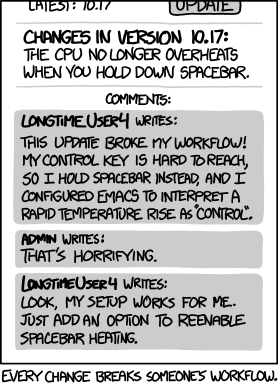
\includegraphics[width=0.3\textwidth]{workflow.png}}
	\end{block}
\end{frame}

\section{When to expect QGIS 3}
\subsection{Overview of the current release cycle}
\begin{frame}{Release cycle}
	\centering{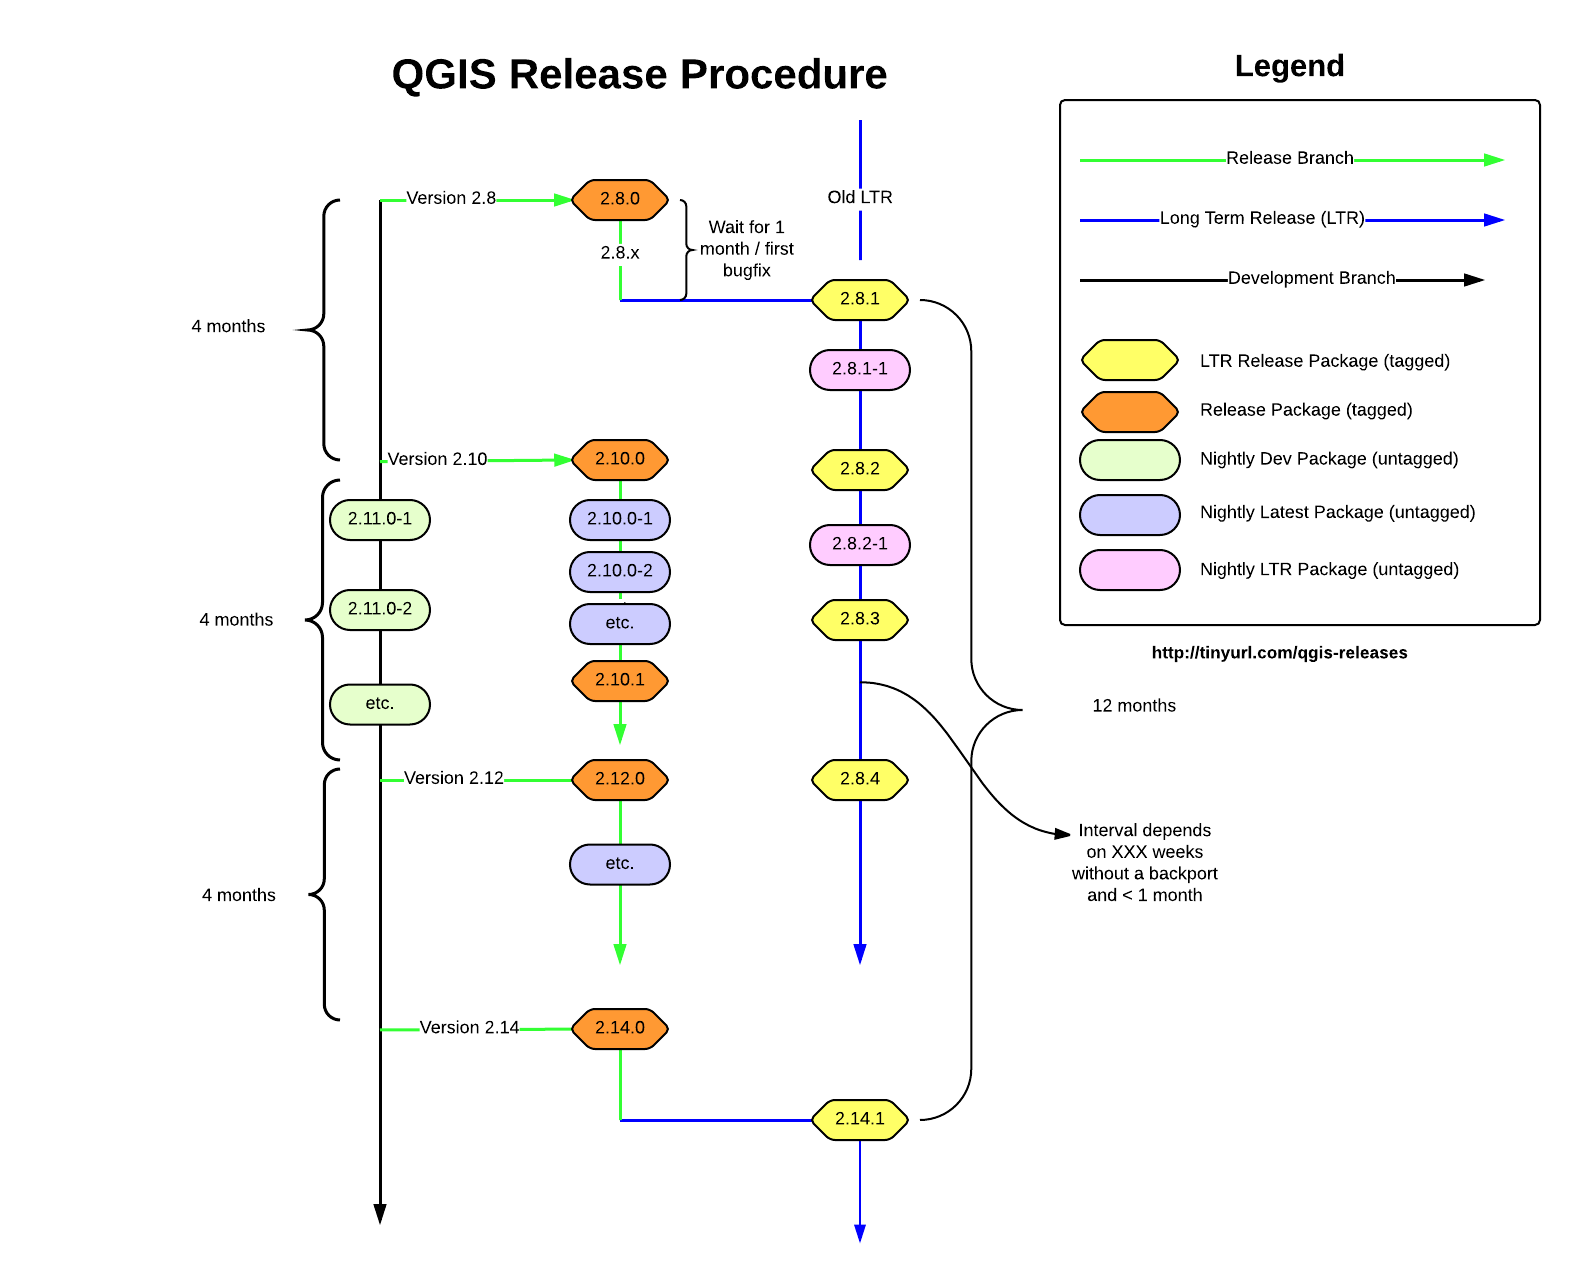
\includegraphics[width=0.8\textwidth]{ae1c0956-523e-11e4-95d9-cea1a3429faf.png}}
\end{frame}

\begin{frame}{Proposed changes}
	\begin{block}{}
		\begin{itemize}
			\item 2.14 remains the last LTR (bugs will be backported to the branch)
			\item 2.18 (until the first 3.0 release)
				\begin{itemize}
					\item will also receive the bug fixes
					\item some new features 
				\end{itemize}
			\item 3.0 likely to be spring/summer 2017
			\item 3.2 will be the next LTR (4 months after 3.0 release)
		\end{itemize}
	\end{block}
\end{frame}

\section{How can you help}

\begin{frame}{How to help QGIS 3.x migration}
\begin{block}{}
	\begin{itemize}
		\item Donate to QGIS.ORG \footnote{http://www.qgis.org/en/site/getinvolved/donations.html}
		\item Test and report bugs
		\item Sponsor bug fixing
	\end{itemize}
\end{block}

\includegraphics[width=0.1\textwidth]{bronze.png} 
\includegraphics[width=0.3\textwidth]{windsor.png} 
\end{frame}


\section{Lutra plan for QGIS 3.0}
\begin{frame}{Our plan for QGIS 3.0}
	\begin{block}{Project and layer registry refactoring}
		\begin{itemize}
			\item Support for multiple projects
			\item Implications/improvements to QGIS Server
		\end{itemize}
	\end{block}
\end{frame}

\begin{frame}{Our plan for QGIS 3.0}
	\begin{block}{Improved Node Tool}
		\begin{itemize}
			\item Work with the Advanced Digitizing Tools 
			\item Editing nodes from multiple layers simultaneously
			\item More responsive and faster
		\end{itemize}
	\end{block}
\end{frame}

\begin{frame}{Our plan for QGIS 3.0}
	\begin{block}{Help with QGIS server refactoring}
		\begin{itemize}
			\item A full PyQGIS application
			\item Tile server
		\end{itemize}
	\end{block}
\end{frame}

\begin{frame}{Our plan for QGIS 3.0}
	\begin{block}{QGIS Mobile}
		\begin{itemize}
			\item Creating a new QGIS Mobile library (based on QGIS Core library):
			\begin{itemize}
			\item Featuring touch optimised GUI components based on Qt Quick
			\item Basic mapping components - map canvas, layer tree (legend), GPS position, scale bar, markers
			\item Support for capturing of new geometries
			\item Display and editing of feature forms
			\item Tools for seamless data sync to/from desktop
		\end{itemize}
		\end{itemize}
	\end{block}
\centering{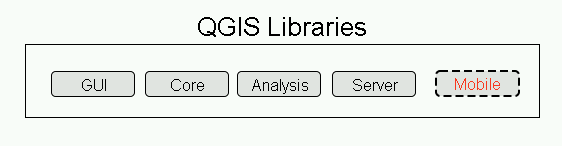
\includegraphics[width=0.6\textwidth]{classes.png}}
\end{frame}